%\documentclass[spanish]{maciarticle}
\documentclass[english]{maciarticle}
%% Si su art\'{\i}culo est\'{a} escrito en ingl\'{e}s debe escribir la opci\'{o}n "english"

\usepackage{amsmath,amsbsy,amscd,amssymb,graphicx,epsfig,color}

%%%%%%%%%%%%%%%%%%%%%%%%%%%%%%%%%%%%%%%%%%%%%
\begin{document}

\title{Monte Carlo Integration: the VEGAS algorithm for Graphics Processing Units}

\author[$a$]{Luis Biedma}
\author[$b$]{Flavio D. Colavecchia}
\affil[$a$]{FAMAF - Universidad Nacional de C\'ordoba,
	           CIEM - CONICET,
               \textcolor{blue}{lbiedma@famaf.unc.edu.ar}}
%
\affil[$b$]{Div. F\'isica At\'omica, Molecular y \'Optica,
	            Centro At\'omico Bariloche,
	            CONICET,
                \textcolor{blue}{flavioc@cab.cnea.gov.ar}}


 \maketitle


\begin{abstract}
This work presents a review and modification of the VEGAS integrating algorithm in Graphics Processing Units. The changes made to the program allow for better performance and use of memory to incorporate more evaluation points, which was an important restriction for the original code on high dimension spaces.
\end{abstract}

\begin{keywords}
GPU, Monte Carlo methods, VEGAS
\end{keywords}

\begin{mathsubclass}
65C05 - 68M20
\end{mathsubclass}


{\thispagestyle{empty}} %NO BORRE ESTA LINEA



%%===============================
\section{Introduction}
%%===============================

Monte Carlo methods are a wide and well known class of computational algorithms that rely on repeated random samplings to get numerical results. One of their main applications is the numerical integration of functions in problems ranging from particle physics\cite{lhc} to cosmology\cite{cosmo}. The usual working pattern for these algorithms is:

\begin{itemize}
	\item Definition of a possible input domain.
	\item Generation of random inputs from a \textit{probability distribution} over the domain.
	\item \textit{Deterministic} computations over the inputs.
	\item Results gathering.
\end{itemize}

Since its creation, lots of efforts have been made in order to boost Monte Carlo methods performance, especially concerning the minimization of numerical errors and the algorithm's speed, trying to adapt them to every new coming computing architecture, including graphics processing units (GPUs), by creating different alternatives for them\cite{montesurvey}.

One of those alternatives is the VEGAS algorithm, created by G.P. Lepage\cite{vegas}. It is based in the concept of \textit{importance sampling}: It samples points from the probability distribution described by the function $\|f\|$ to be integrated, so that the sampling points are concentrated in the regions that make the largest contribution to the integral. VEGAS is based on an iterative and adaptive Monte Carlo scheme: each axis of variable is divided into grids, dividing the integration space into hypercubes. Monte Carlo integrations are performed on each hypercube and the variances from hypercubes are used to adapt the shape of the grids, which will be used in the next iteration, reducing the variance of the total integral at each step.

The aim of this work is to improve the code of a multi-dimensional VEGAS algorithm, which uses GPUs, created by J. Kanzaki in 2011\cite{kanzaki}.

\section{The Initial Program} 
Kanzaki's code can be found at \textcolor{blue}{http://madgraph.kek.jp/KEK/GPU/gVEGAS/example/} and is used as the basis for the new program. It is written in CUDA language, adapted from FORTRAN code created originally by Lepage\cite{lepagecode}. There is a single and double precision version available in the webpage. The steps followed by the program in each iteration are:

\begin{enumerate}
	\item Generation of the integration space, dividing it into hypercubes.
	\item \vspace{-0.3cm} That data is sent to the GPU, where the function evaluations are performed and the information per hypercube is gathered.
	\item \vspace{-0.3cm} These results are sent back to the CPU, where weighted averages, approximation errors and the reallocation of the grid are performed.
	\item \vspace{-0.6cm} If the amount of iterations is reached or a minimum value of error is obtained, the program stops.
\end{enumerate} 

Although this code has great performance relative to the first stages of VEGAS (evaluating a function in lots of different points in space on GPUs is an embarrasingly parallel task), there are still some issues that are addresed in this work.

There is a considerable amount of data moved between GPU and CPU. The code generates an array of evaluations (one for each point) and also needs to store information regarding the grid box the point is occupying, for each dimension, in the integration space. So, for every evaluation point, the program needs (\textit{dim}+1) * 4 bytes (in single precision) of RAM, where \textit{dim} is the dimension of the integration space. When working on GPUs, memory management is an important issue and it is not properly addressed in this code.

The complete weighted averages are computed in the CPU, but it can be also performed in GPU, because the \textit{reduction} operation is easy to parallelize. The grid evaluation can also work in parallel.

\section{Modifications}

The new CUDA kernel performs the values (and their squares) reduction, aided by the \textit{atomicAdd} instruction\cite{cudaprog} and also takes the data to an histogram array, which is passed to the CPU to obtain the grid rearrangement for the next iteration. In conclusion, this code merges steps 2 and 3 for the original program.
This array has a fixed (very small relative to the amount of points generated) size,
so there aren't any memory issues.

An important note is that the original code passes single precision numbers to double when it computes the weighted averages for the integrals. The new code uses only single precision since it works with the \textit{atomicAdd} instruction and it is only available for single precision in the Maxwell architecture, which was the one used for this work.

The entire code is hosted at \textcolor{blue}{https://github.com/lbiedma/gVegascp}.

\section{Numerical Results}

The performance experiments are divided in two stages: pure speed comparison and numerical correctness. They were run on the following hardware:

\begin{center}
	\begin{tabular}{ll}
		\hline
		\textbf{CPU} & 2x Intel(R) Xeon(R) CPU E5-2620 (12 cores at 2.40 GHz) \\
		\textbf{Memory} & 128 GB DDR3 \\
		\textbf{GPU} & NVIDIA GeForce GTX Titan X (12 GB RAM)\\
		\hline
	\end{tabular}
\end{center}



\subsection*{Speed Comparison}

The termination conditions were set at $1 \times 10^{-6}$ for the relative error between estimated integrals per step and 10 as the max amount of iterations. The space dimension $d$ was limited to a maximum of 8 and the amount of points used was increased on each execution from $2^{10}$ to $2^{24}$ (the memory limitations on the original code made it impossible to reach higher dimension numbers). Only for speed comparison purposes, the multi-dimensional paraboloid ($\|x\|^2$) in the $[-1,1]^d$ hypercube was chosen.

The following graph shows the performance of the original and the modified programs, with time normalized by the number of points used and the amount of iterations.

\begin{center}
	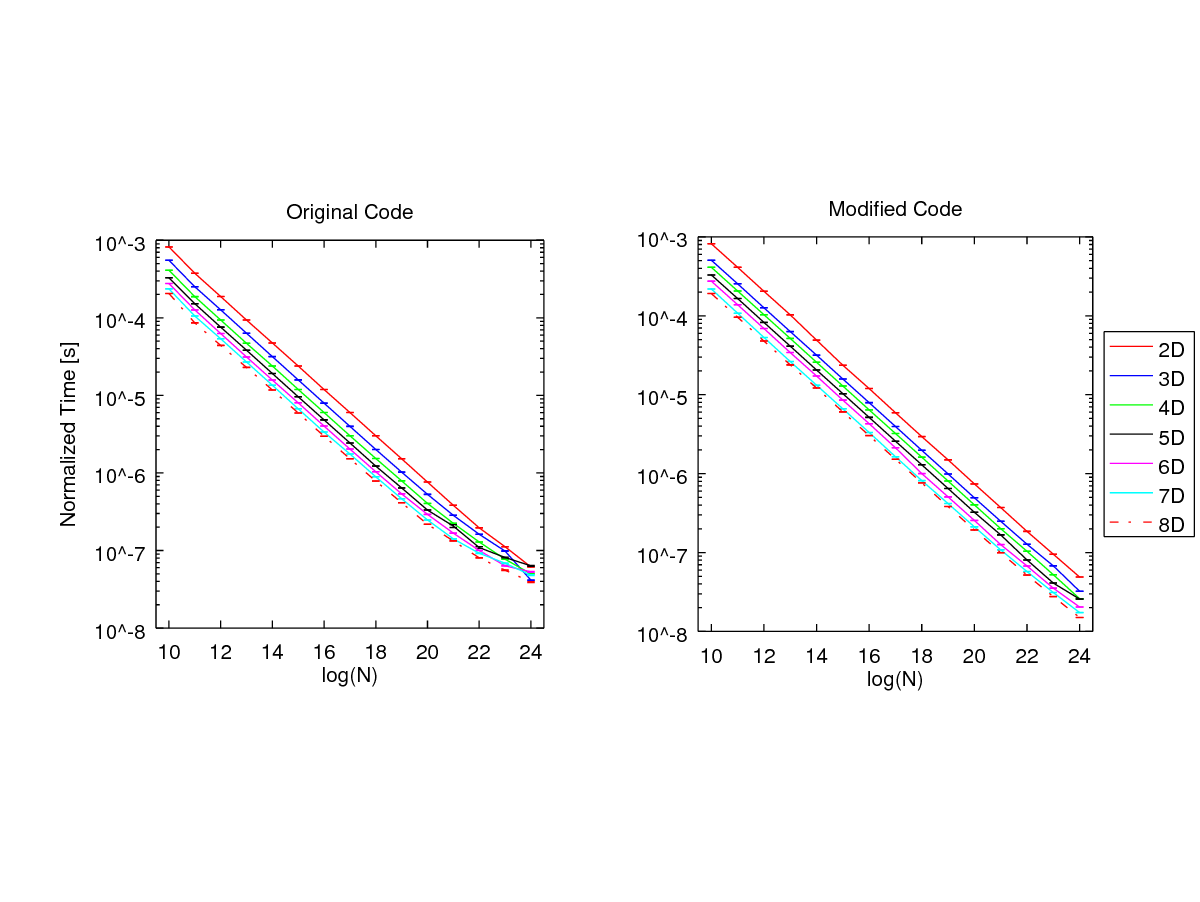
\includegraphics[width = .9\textwidth]{comparison.png}
\end{center}

It can be observed that both programs perform at almost the same speed at first, but the new program continues to maintain a good performance as the amount of function evaluations increases. More points couldn't be evaluated because of memory restrictions for the original code.

\subsection*{Benchmarking}

The numerical correctness tests for the modified program were based on Scilab's testing toolbox for Monte Carlo and Quasi Monte Carlo methods\cite{baudin}. The integral of the functions is zero for every dimension. 17 integrals from this toolbox were tested, with dimensions ranging from $d=6,\dots, 12$, and evaluation points $n = 262144, 524288, 1048576, \dots, 67108864$ (powers of 2 from 18 up to 26) in the $[0, 1]^d$ hypercube. The random number generator used was a version of XORSHIFT available in the repository.

For each function, the success rate of the program (percentage of integrals along with their standard deviations that are equal to zero) and a normalized average computation time is reported.

%\begin{center}
%	\begin{tabular}{ccc}
%		\hline
%		Points & Rate & Time [s] \\
%		\hline
%		$2^{18}$ & 42.0\% & $4.133 \times 10^{-9}$\\
%		$2^{19}$ & 52.4\% & $2.323 \times 10^{-9}$\\
%		$2^{20}$ & 58.8\% & $2.095 \times 10^{-9}$\\
%		$2^{21}$ & 80.7\% & $1.463 \times 10^{-9}$\\
%		$2^{22}$ & 68.1\% & $1.388 \times 10^{-9}$\\
%		$2^{23}$ & 68.9\% & $1.304 \times 10^{-9}$\\
%		$2^{24}$ & 67.2\% & $1.298 \times 10^{-9}$\\
%		$2^{25}$ & 77.3\% & $1.278 \times 10^{-9}$\\
%		$2^{26}$ & 67.2\% & $1.214 \times 10^{-9}$\\
%		\hline
%	\end{tabular}
%\end{center}

\begin{center}
	\begin{tabular}{ccc}
		\hline
		Function & Rate & Time[s] \\
		\hline
				SUM & 95.2\% & $1.715 \times 10^{-9}$\\
				SQSUM & 92.1\% & $1.718 \times 10^{-9}$\\
				SUMSQROOT & 92.1\% & $1.814 \times 10^{-9}$\\
				PRODONES & 71.4\% & $1.675 \times 10^{-9}$\\
				PRODEXP & 49.2\% & $1.908 \times 10^{-9}$\\
				PRODCUB & 42.8\% & $1.712 \times 10^{-9}$\\
				PRODX & 38.1\% & $1.716 \times 10^{-9}$\\
				SUMFIFJ & 38.1\% & $2.010 \times 10^{-9}$\\
				SUMF1FJ & 46.0\% & $2.551 \times 10^{-9}$\\
				HELLEKALEK & 100\% & $1.841 \times 10^{-9}$\\
				ROOSARNOLD1 & 66.7\% & $1.670 \times 10^{-9}$\\
				ROOSARNOLD2 & 30.2\% & $1.739 \times 10^{-9}$\\
				ROOSARNOLD3 & 34.9\% & $1.888 \times 10^{-9}$\\
				RST1 & 57.1\% & $1.722 \times 10^{-9}$\\
				SOBOLPROD & 95.3\% & $1.858 \times 10^{-9}$\\
				OSCILL & 84.1\% & $1.771 \times 10^{-9}$\\
				PRPEAK & 68.3\% & $1.824 \times 10^{-9}$\\
		
	\end{tabular}
\end{center}

It can be observed that the program performs well on half of the functions in the toolbox. These results seem disappointing, but the cause for this problem may be a bad combination of dimensions and evaluation points, since some of the functions present a big amount of extremes, which grow with the dimension of the integration space. A finely tuned configuration of these parameters may present better results in the future, along with a different random number generator.


\section{Summary and Outlooks}
The modifications applied to the original program allowed it to perform at a higher speed for big problems and manage memory in a better way, which is an important issue when working with GPUs, since RAM is highly limited.

NVIDIA's new GPU architecture (Pascal) incorporates the \textit{atomicAdd} instruction for double precision numbers\cite{pascal}, this will be really useful to achieve high performance in double real and complex precision computations, and may be the subject of future work. 

\section*{Acknowledgments}
The first author would like to thank Nicol\'as Wolovick and Carlos Bederi\'an, of the
GPGPU Computing Group in FAMAF, Universidad Nacional de C\'ordoba, for their Parallel Programming course and its notes\cite{cp2016}, where this work began.


%%=========================================
\begin{thebibliography}{1}
%%=========================================
\bibitem{lhc} {\sc{S. Wertz}},
\emph{The Matrix Element Method at the LHC: Status and prospects for Run II},
17th International Workshop on Advanced Computing and Analysis Techniques in Physics Research, 2016.

\bibitem{cosmo} {\sc{A. Taruya}},
\emph{Constructing perturbation theory kernels for large-scale structure in generalized cosmologies},
Physical Review D - Particles, Fields, Gravitation and Cosmology, 2016.

\bibitem{montesurvey} {\sc{J.H.Halton}},
\emph{A Retrospective and Prospective Survey of the Monte Carlo Method}
SIAM Review, 1970.

\bibitem{vegas} {\sc{G.P. Lepage}},
\emph{A new algorithm for adaptive multidimensional integration},
Journal of Computational Physics, 1978.

\bibitem{kanzaki} {\sc{J. Kanzaki}},
{\em Monte Carlo integration on GPU},
The European Physical Journal C, 2011.

\bibitem{lepagecode} {\sc{G.P. Lepage}},
{\em VEGAS: An Adaptive Multi-dimensional Integration Program},
Cornell preprint CLNS, 1980.

\bibitem{cudaprog} {\sc{NVIDIA}}, {\em CUDA C Programming Guide},
\textcolor{blue}{http://docs.nvidia.com/cuda/cuda-c-programming-guide}.

\bibitem{pascal} {\sc{NVIDIA}}, {\em CUDA Pascal Tuning Guide} \textcolor{blue}{http://docs.nvidia.com/cuda/pascal-tuning-guide}.

\bibitem{baudin} {\sc{M. Baudin}},
\emph{The Integration Test Problems Toolbox, version 0.1},
Scilab, 2010.

\bibitem{cp2016} {\sc{Nicolas Wolovick}},
{\em Computaci\'on Paralela 2016}, \textcolor{blue}{https://cs.famaf.unc.edu.ar/\~nicolasw/Docencia/CP/2016/index.html},
FAMAF - UNC, 2016.
\end{thebibliography}

\end{document}
